%!TEX encoding = UTF-8 Unicode
%!TEX root = ./../main.tex
%!TEX TS-program = xelatex

\chapter{Risultati sperimentali} % 5th chapter title
\label{cap:sette}
La valutazione delle \textit{performances} di un algoritmo di \ac{GI} possono essere influenzate sia positivamente che negativamente da alcuni fattori come già evidenziato in \ref{sec:gensam}. Uno di questi fattori è la complessità del \ac{DFA} target con cui si intende\cite{Stamina10}:
\begin{itemize}
\item numero di stati
\item dimensione dell'alfabeto
\item la lunghezza del più lungo dei cammini minimi dallo stato iniziale a qualunque altro stato
\item il numero di transizioni
\item il numero di transizioni totali\footnote{ (escluse quelle che vanno nello stato pozzo, altrimenti sarebbero tutte in egual numero in un \ac{DFA})}
\end{itemize}
Anche la dimensione del \textit{training set} e del \textit{test set} è rilevante e quindi è necessario scandagliare il comportamento dell'algoritmo al variare della dimensionalità di questi parametri. Attenendosi all'impostazione della competizione STAMINA \cite{Stamina10} si è scelto di [INSERIRE DIMENSIONI ALFABETO STATI TRAINING SET]

Nell'effettuazione degli esperimenti è necessario tenerne conto onde evitare dei risultati pessimisticamente o ottimisticamente \textit{biased}. 

\section{Dataset}
In letteratura si trovano molti algoritmi innovativi di \ac{GI} ,dei quali non si conoscono ancora le caratteristiche, che sono preventivamente testati su dei linguaggi regolari ''non banali'' ma relativamente semplici. In un secondo momento i limiti dell'algoritmo sono testati contro linguaggi più complessi che ricalcano da vicino la complessità degli automi testati nelle varie competizioni di \ac{GI} o su dataser reali. Per le finalità di questo lavoro si è scelto di perseguire questa strada.

\subsection{Tomita Dataset}
Tomita in \cite{Tomita82} definisce sette linguagi regolari, da lui usati per provare il suo algoritmo di inferenza grammaticale basato sulla tecnica di hill–climbing. Succesivamente in \cite{Dupont94}, questo insieme viene ampliato aggiungenedo altri otto linguaggi regolari. L'elenco completo dei quindici linguaggi regolari si trova in tabella \ref{tab:tom} e raggiunge un massimo di sei stati con $L_{10}$ e l'alfabeto è binario tranne in due casi, $L_{9}$ e $L_{15}$ , in cui $|\Sigma|$ = 3 . Alcuni di essi sono descritti dall’espressione regolare corrispondente. Nei casi in cui l’espressione regolare fosse troppo complicata al fine di capire immediatamente la “regolarità” del linguaggio, si è preferito fornirne una descrizione informale. Ad esempio l’espressione regolare per il linguaggio $L_6$ è $((a(ab)^{*}  (b|aa))|(b(ba)^{*} (a|bb)))^{*}$ : non è immediato riconoscere in questo caso la regolarità aritmetica posseduta dal linguaggio, costituito da tutte le stringhe in cui il numero dei caratteri $a$ differisce dal numero dei caratteri $b$ per un numero divisibile per tre.
 
\begin{table}[htp]
\centering 
\begin{tabular}{|c|M{0.75\textwidth}|} 
\hline
$L_{1}$ & $a^{*}$  \\
 \hline
 $L_{2}$ & $(ab)^{*}$  \\
 \hline
 $L_{3}$ & Ogni stringa che non contiene un numero dispari di a consecutivi dopo un numero dispari di b consecutivi  \\
 \hline   
 $L_{4}$ & Ogni stringa che non contiene la sottostringa aaa  \\
 \hline
 $L_{5}$ & Ogni stringa che contiene un numero pari di a ed un numero pari di b  \\
 \hline   
  $L_{6}$ & Ogni stringa in cui il numero di a contenute differisce dal numero di b
contenute per un numero divisibile per tre.  \\
 \hline  
 $L_{7}$ & $a^*b^*a^*b^*$  \\
 \hline
 $L_{8}$ & $a^*b$  \\
 \hline
  $L_{9}$ & $(a^*+c^*)b^*$  \\
 \hline
 $L_{10}$ & $(aa)^*(bbb)^*$  \\
 \hline
 $L_{11}$ & Ogni stringa che contiene un numero pari di a ed un numero dispari di b \\
 \hline 
 $L_{12}$ & $a(aa)^*b$ \\
 \hline     
 $L_{13}$ & Ogni stringa che contiene un numero pari di a \\
 \hline       
 $L_{14}$ & $(aa)^*ba^*$ \\
 \hline 
 $L_{15}$ & $bc^*b+ac^*a$ \\
 \hline 
\end{tabular}

 \caption[Linguaggi Tomita]{Linguaggi Tomita}
\label{tab:tom}
\end{table} 

\begin{figure}[htp]
\centering
\subfloat[$L_1$][\label{sub:tom1}]
{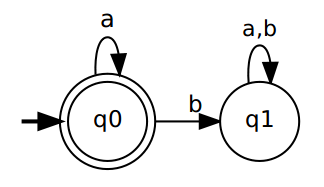
\includegraphics[width=.40\textwidth,height=4cm,keepaspectratio]{Tomita1}} \quad
\subfloat[$L_2$][\label{sub:tom2}]
{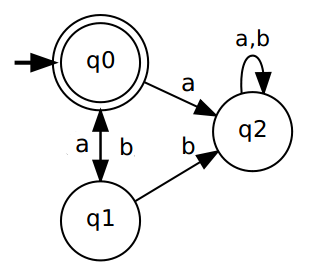
\includegraphics[width=.45\textwidth,height=4cm,keepaspectratio]{Tomita2}}\\

\subfloat[$L_3$][\label{sub:tom3}]
{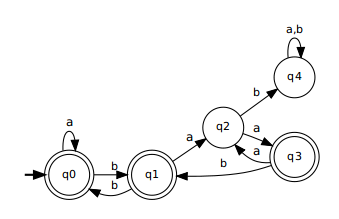
\includegraphics[width=.45\textwidth,height=4cm,keepaspectratio]{Tomita3}} \quad
\subfloat[$L_4$][\label{sub:tom4}]
{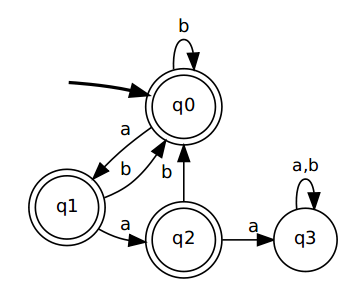
\includegraphics[width=.45\textwidth,height=4cm,keepaspectratio]{Tomita4}}\\

\subfloat[$L_5$][\label{sub:tom5}]
{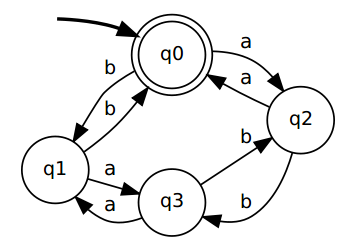
\includegraphics[width=.45\textwidth,height=4cm,keepaspectratio]{Tomita5}} \quad
\subfloat[$L_6$][\label{sub:tom6}]
{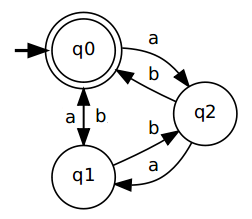
\includegraphics[width=.45\textwidth,height=4cm,keepaspectratio]{Tomita6}}\\

\subfloat[$L_7$][\label{sub:tom7}]
{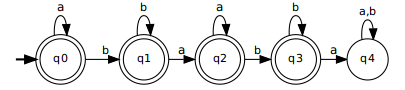
\includegraphics[width=.50\textwidth,height=4cm,keepaspectratio]{Tomita7}} \quad
\subfloat[$L_8$][\label{sub:tom8}]
{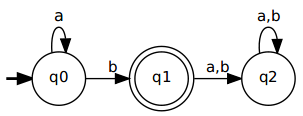
\includegraphics[width=.40\textwidth,height=4cm,keepaspectratio]{Tomita8}}\\
\caption{Linguaggi di Tomita}
\label{fig:ltom1}
\end{figure} 

\begin{figure}[htp]\ContinuedFloat
\centering
\subfloat[$L_9$][\label{sub:tom9}]
{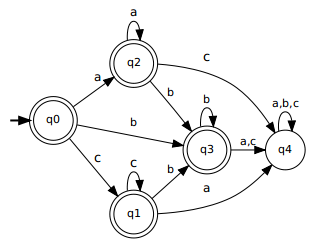
\includegraphics[width=.45\textwidth,height=4cm,keepaspectratio]{Tomita9}} \quad
\subfloat[$L_10$][\label{sub:tom10}]
{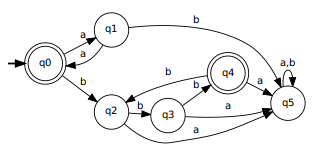
\includegraphics[width=.45\textwidth,height=4cm,keepaspectratio]{Tomita10}}\\

\subfloat[$L_11$][\label{sub:tom11}]
{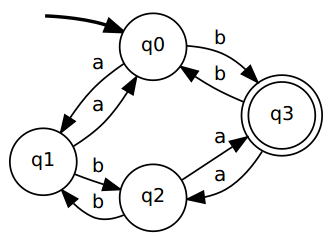
\includegraphics[width=.45\textwidth,height=4cm,keepaspectratio]{Tomita11}} \quad
\subfloat[$L_12$][\label{sub:tom12}]
{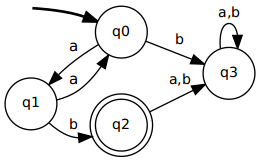
\includegraphics[width=.45\textwidth,height=4cm,keepaspectratio]{Tomita12}}\\

\subfloat[$L_13$][\label{sub:tom13}]
{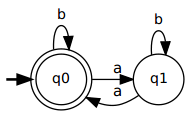
\includegraphics[width=.45\textwidth,height=4cm,keepaspectratio]{Tomita13}} \quad
\subfloat[$L_14$][\label{sub:tom14}]
{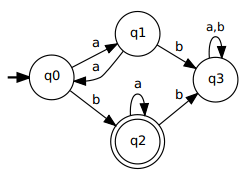
\includegraphics[width=.45\textwidth,height=4cm,keepaspectratio]{Tomita14}}\\

\subfloat[$L_15$][\label{sub:tom15}]
{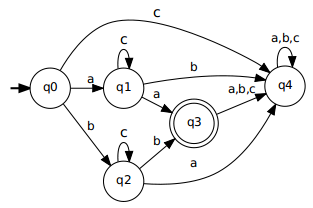
\includegraphics[width=.45\textwidth,height=4cm,keepaspectratio]{Tomita15}}

\caption{Linguaggi di Tomita}
\label{fig:ltom2}
\end{figure} 
todo:
Riorganizzare quanto sopra introducendo prima Tomita.
Descrivi Tomita
Giustifica risultati anche perchè si approssimano anche le MQ.
Fai vedere che comunque esistono dei modelli complessi con cui si hanno buoni risultati (anche se la complessità è tutta da vedeere e non è decisa solo dagli stati dall'alfabeto e dalla profondità, ma dipende anche da quanto sono buoni i campioni estratti col random walk).
Illustra i set di esperimenti e i risultati.